\documentclass[]{article}
\usepackage[hidelinks]{hyperref}
\usepackage{graphicx}
%opening
\title{Building a better Sketch-Y-Etch}
\author{Sensored Hacker}

\begin{document}

\maketitle

\begin{abstract}
Initial versions of the sketch-y-etch had issues related to haphazard planing, and inconsistent use of parts. It has been two years since the initial creation filled the Bangor Makerspace with retro drawing for all, and we have heard many things about 
what makes the sketch-y-etch hard to use. Here in v2, we are going to try an fix the issues. 
\end{abstract}

\section*{ISSUES:}
\begin{itemize}
	\item \textbf{Drawing Performance:} Performance was limited by encoder issues.
	\item \textbf{Build Quality:} V1 used available parts with no specific plan for integration, negatively affecting the overall experience.
	\item \textbf{Stability:} The wobble made drawing difficult. While the Sketch-Y-Etch has never tipped over, it feels like it could—and that can be fixed.
%	\item \textbf{Portability:} Portability was never a design goal of V1 but can be improved in V2.
	\item \textbf{Documentation:} Existing documentation focused on the history and developer notes but lacked detailed build instructions.
	\item \textbf{Bill of Materials:} A BOM was non-existent in V1. Not everyone has a stockpile of miscellaneous computer parts.
\end{itemize}

\section*{Improvements}

\begin{itemize}
	\item \textbf{Improved Components:} A concerted effort was made to use higher-quality parts throughout the build.
	\item \textbf{Specialized Hardware:} A new conceptual design in v2 maintains compatibility with a wide range of hardware and platforms, while offering many new design options.
	\item \textbf{Focused Documentation:} We want you to build your own Sketch-Y-Etch! A detailed tutorial is now available to guide you through the process.
	\item \textbf{New Features:} More colors, adjustable pen size, dynamic scaling, and additional enhancements.
	\item \textbf{Bill of Materials:} All required parts can be easily acquired, with a total estimated cost of about \$50.
\end{itemize}

\section*{Let's Build It!}

To begin building your Sketch-Y-Etch, you will need a set of materials and tools.  
The Bangor Makerspace offers complete kits for purchase if you are interested, or you can source your own components independently.

\subsection*{Required Tools}

Basic tools required for assembly include:
\begin{itemize}
	\item Screwdrivers
	\item 3D printer
	\item Wire cutters
	\item Soldering station
	\item Drill and drill bits
	\item Personal protective equipment (PPE)
\end{itemize}

\subsection*{Electronic Components}

The Bangor Makerspace developed the HDMI-TAP specifically for this project. While its use is highly recommended for simplicity and reliability, it is also possible to build a compatible alternative at relatively low cost.\\

This project utilizes Qwiic connectors for inter-device communication over I\textsuperscript{2}C.  
A common practice in electronics is to color-code wires according to their function. Although wire insulation color does not affect circuit operation, following a standard color convention greatly simplifies visual inspection and troubleshooting.

In this project, the following color scheme is used:

\begin{itemize}
	\item \textbf{Red:} +5VDC (power)
	\item \textbf{Black:} Ground (common)
	\item \textbf{Blue:} SDA (I\textsuperscript{2}C data line)
	\item \textbf{Yellow:} SCL (I\textsuperscript{2}C clock line)
\end{itemize}

As a mnemonic, you can remember that \textit{yellow} (like the sun on a sundial) represents the clock signal.

This color convention matches the standards used by Adafruit STEMMA QT and SparkFun Qwiic connect systems, utilized in this project.

\subsection*{Bill of Materials}

\begin{center}
	\begin{tabular}{|l|l|c|l|}
		\hline
		\textbf{Item} & \textbf{Part Number / Name} & \textbf{Qty} & \textbf{Notes} \\
		\hline
		Rotary Encoder & Adafruit Seesaw Encoder   & 4 & I2C, with built-in pullups \\
		Display        & HDMI Monitor              & 1 & Any 1080p-capable screen \\
		Cables         & Assorted Qwiic Wires      & 5 & Male-male and male-female \\
		Knobs          & Custom 3D-Printed Knobs   & 1 & STL files available \\
		Computer       & Any with HDMI Output      & 1 & Laptop, desktop, or SBC \\
		HDMI-TAP       & v2 w/qwiic connects	   & 1 &  easy access HDMI i2c bus.\\
		
		\hline
	\end{tabular}
\end{center}



\section*{Download the Code}

If you have not yet installed Python 3, download and install it now.  
You will also need the \texttt{numpy} and \texttt{smbus2} libraries, which can be installed with:

\begin{verbatim}
	pip install numpy smbus2
\end{verbatim}

Download the source repository for the Sketch-Y-Etch project, available at:  
\url{https://github.com/FOSSBOSS/SketchyEtch}

Once you have the repository, extract it if necessary, and navigate to the \texttt{v2\_WIP} folder.  
In your IDE of choice, try running \texttt{SketchyV2\_WIP.py}.

If you encounter import errors, you may be missing required libraries, or your Python 3 path may be incorrect.

\begin{figure}[ht]
	\centering
	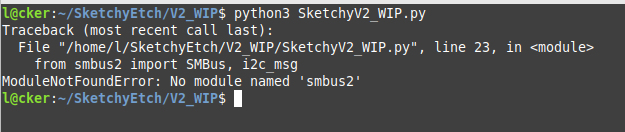
\includegraphics[width=0.8\textwidth]{missing.png}
	\caption{Missing \texttt{smbus2} library error example.}
	\label{fig:missing_smbus2}
\end{figure}

\section*{Embrace Complexity}

This project has many possible configurations. Here are two basic setups you might consider:

\begin{enumerate}
	\item Connect a computer to the Sketch-Y-Etch, then to a display screen.
	\item Connect a laptop's HDMI output directly to the Sketch-Y-Etch.
\end{enumerate}

Many possibilities and functionalities exist at this stage. The zeitgeist of this project is to embrace experimentation, and creativity with flexibility. Take some time to consider how you want to configure your Sketch-Y-Etch.

While video pass-through is an option, if you have multiple display outputs, you may route your controls in various ways. You might choose to embed the Sketch-Y-Etch into a TV, build a standalone control panel, make multiple controllers on one computer, use a projector, or simply connect via a laptop using HDMI as a control bus only.\\

Is HDMI strictly required? Not necessarily. HDMI is modern and widely available, but it is not the only option. Other video or data interfaces could be adapted with additional development effort. Adaptions may change the path of these instructions, which should conceptually work regardless of your desired implementations. I am however not going to write a new tutorial for every conceivable build path, or video technology in existence. \\

Please keep in mind: this project remains experimental. It is not intended as a polished, professional consumer product.  
While it is feasible to create a more plug-and-play experience, the practical setup will depend heavily on the specific hardware you have available.
This flexibility can be confusing at first, but the key is to clearly define what you want to build before you start building it.

\subsection*{Optional Steps}

These steps are not strictly required but are highly recommended to simplify testing and setup. 3D printing the knobs, and experimental build platform may take approximately an hour of printing, depending on your printer. Print 4 knobs, and 1 table. Please note that the current knob.stl file is sized for the encoders used in this project, if you are using some other unspecified component you may need to adjust the models to meet your specific needs. 

\begin{enumerate}
	\item 3D print the \texttt{table.scad} build platform and install your devices onto it.
	\item Drill or melt holes into the table  to match your layout preferences. 
	\item Install the knobs by pushing them on to the encoder shafts. Using alternate knobs is also acceptable, we're just trying to make the encoders easy to use.
	\item Test and verify all hardware and software functionality using the build platform before embedding the electronics into a TV.
\end{enumerate}

\section*{Wiring}
Assuming you are following along with building the test platform first for testing, and your 4 rotary encoders are now installed, flip the table to view the encoders for wiring.
The encoders have directionality, which may be counter intuitive. There is an input side, and an output side. If looking at the underside of the encoder, with the LED at the top, or away from you, the input port is on the left, and the output qwiic connect port is on the right. You may opt to label the ports I for input and O for output. When connecting the encoders, you will connect from the output of the first encoder to the input of the next encoder in line. 
\begin{figure}[ht]
	\centering
	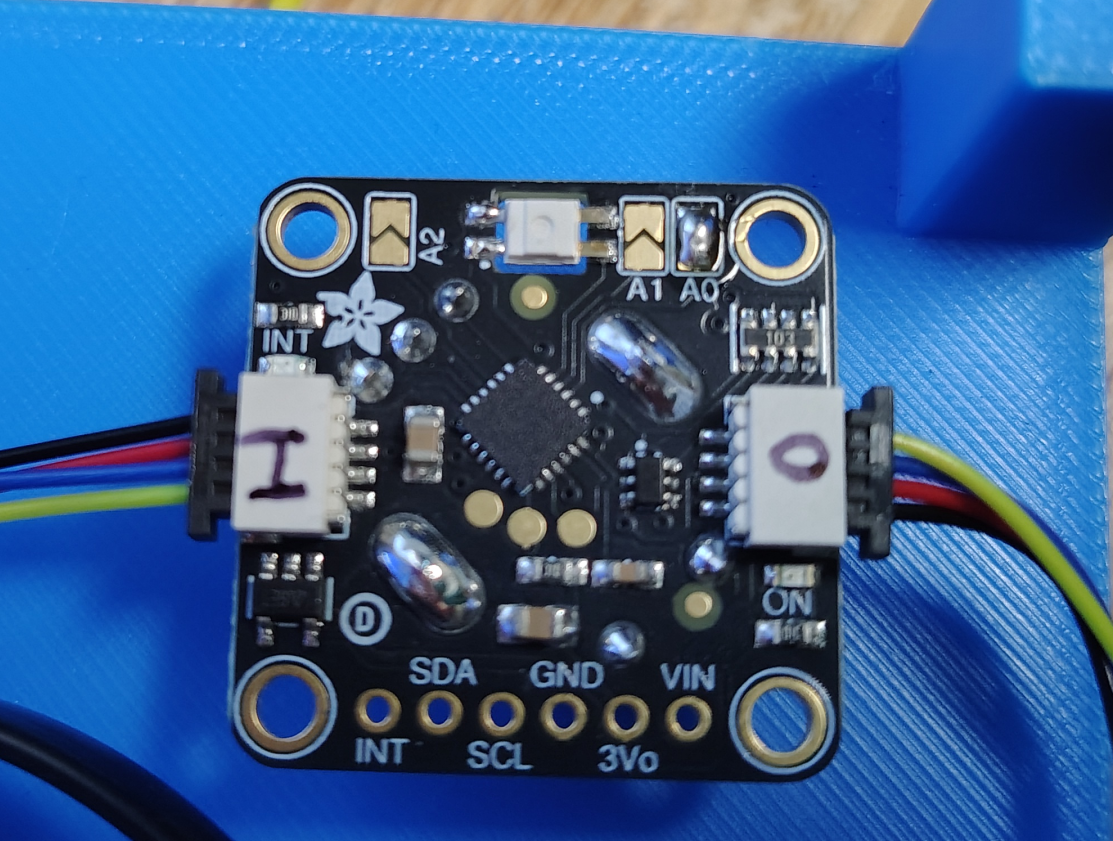
\includegraphics[width=0.8\textwidth]{underside.png}
	%	\caption{flipside \texttt{encoder underside} }
	\label{fig:encoder_underside}
\end{figure}
Here, you can observe the exposed A0, A1, and A2 pads. These pads control the I\textsuperscript{2}C addresses your encoders use to communicate on the bus. 
By default, all pads are disconnected, which is how the encoders are shipped from the factory. The default I\textsuperscript{2}C address is \texttt{0x36}.

By bridging these pads with solder, you manually set the device's address. You can attach your encoders in any order; however, each encoder must have a unique address. Up to eight address combinations are possible.
Please note that whichever addresses you assign must be configured correctly in the software to ensure that each encoder performs its designated function.
 
\begin{figure}[ht]
	\centering
	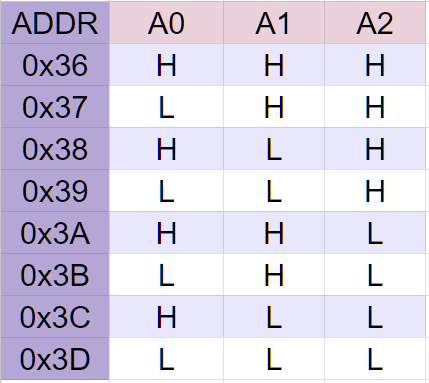
\includegraphics[width=0.8\textwidth]{rotaryEncTable.png}
	\caption{Encoder addresses \texttt{Empty pad is high by default} }
	\label{fig:address asignments}
	\end{figure}

Once you have assigned your 4 distinct addresses by soldering, record those addresses, and their respective functions per your board layout. You will need this information when you go to adapt the SketchyEtch.py code to your specific installation.

\section*{More wiring}



\section*{Inspect}
Inspection is an important step in every electronics project. Mistakes happen, the world is a distracting place, and the fragility of human existence can lead to some unfortunate side effect. Your electronics projects do not need to suffer from this. Look for loose wires, stray strands of wire poking out of terminals, connectors ajar,  messy incoherent wiring... if you can spot problems before they start, it will be safer, and less confusing later. If everything on your test rig looks good, try plugging it in.\\ projects rarely work perfectly the first time around, even with expertly drafted and bespoke instructions. 

Plug your test rig in. Fire? unplug it.\\No fire? no smells? \\ Great!! you have passed the first step of electronics tinkering!
Did your externally attach monitor resume video playback? Did the power lights on the encoders illuminate?

\begin{figure}[ht]
	\centering
	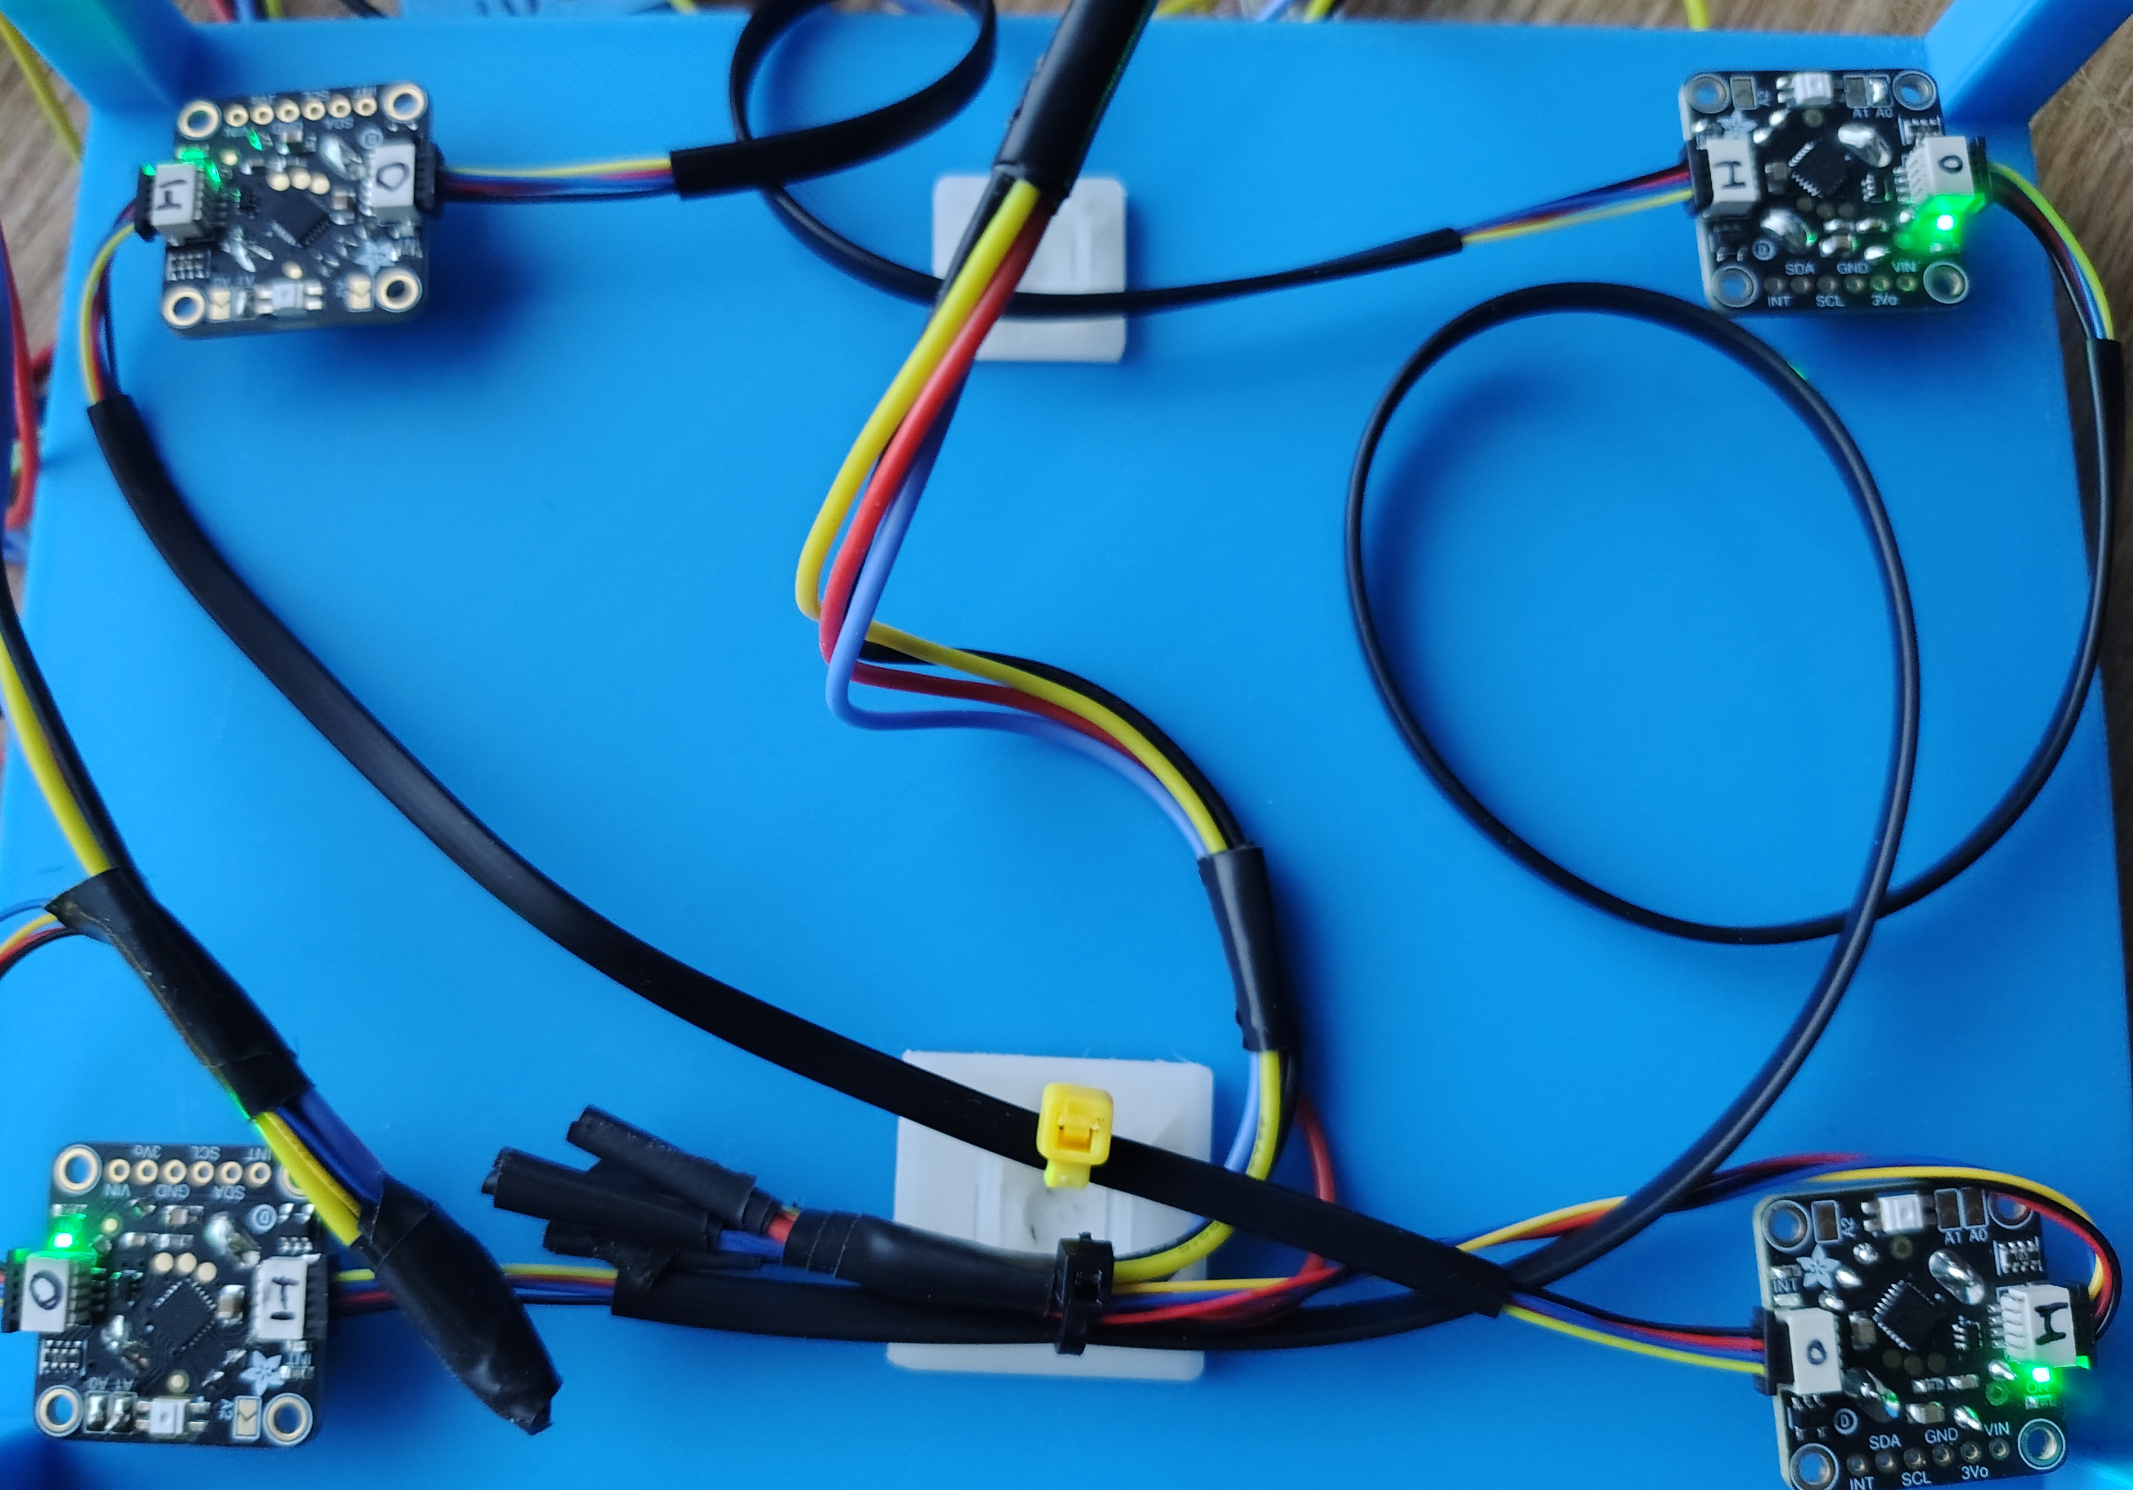
\includegraphics[width=0.8\textwidth]{noFire.png}
	\caption{Lights on! \texttt{no fire!} }
	\label{fig:looks_good}
\end{figure}

If every thing seems to be working, then lets proceed. 
If you start to smell something, or your computer begins to behave erratically, I would suspect the newly attached experimental electronics project, and unplug it as best practice. 
 
\section*{Install Hardware}
% dont forget to write about the ADC!
\section*{Test Hardware}

\section*{Adapt the code}

\section*{Play Time!}

\section*{Troubleshooting}

\section*{Contact}
\begin{enumerate}
\item You love this project, and want to contribute!
\item You have commentary about this document, project, code and want further detail.
\item Complaints.
\end{enumerate}
\section*{Recommended Software}

The only essential software requirement for the Sketch-Y-Etch is a working installation of Python 3:

\begin{itemize}
	\item Python 3: \url{https://www.python.org}
\end{itemize}

\subsection*{Helpful Tools}

The Sketch-Y-Etch was developed primarily on Linux using Python 3 alongside a variety of additional software tools:

\begin{itemize}
	\item OpenSCAD ( for 3D design ): \url{https://openscad.org}
	\item Geany ( lightweight code editor ): \url{https://www.geany.org}
	\item KiCad ( PCB design and schematic capture ): \url{https://www.kicad.org}
	\item i2c-tools ( I\textsuperscript{2}C communication utilities ): \url{https://archive.kernel.org/oldwiki/i2c.wiki.kernel.org/index.php/I2C_Tools.html}
\end{itemize}

While the design should, in principle, work on any operating system, platform-specific nuances have not been extensively tested.  
The tools listed above reflect the preferences of the original developer. Although not strictly required, they are highly recommended for a smoother and more educational development experience.

\section*{References}

\begin{itemize}
	\item Turtle Graphics API (Python Standard Library): \url{https://docs.python.org/3/library/turtle.html}
	\item Smbus2 (Python I\textsuperscript{2}C library) : \url{https://pypi.org/project/smbus2}
	\item I\textsuperscript{2}C Implementation Guide (SparkFun): \url{https://learn.sparkfun.com/tutorials/i2c/all}
	\item Adafruit encoder pinouts \url{https://learn.adafruit.com/adafruit-i2c-qt-rotary-encoder/pinouts}
	\item Adafruit Seesaw Library: \url{https://github.com/adafruit/Adafruit_Seesaw}
	\item Component Datasheets: Included in this repository.
	\item The Book of I\textsuperscript{2}C by Randal Hyde \url{https://nostarch.com/book-i%C2%B2c}
\end{itemize}

All references are provided for educational purposes. They are not required to complete the project but may offer valuable background information.


\end{document}
